\usetikzlibrary{arrows.meta,calc,shapes,decorations.pathreplacing,patterns}
\providecommand{\computer}{%
    
\includegraphics[width=1cm]{../common/Noun_project_216.pdf}
}
\providecommand{\switch}{%
    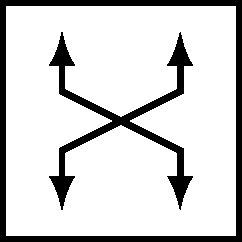
\includegraphics[width=0.9cm]{../common/fig-switch.pdf}
}
\providecommand{\router}{%
    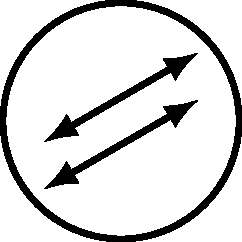
\includegraphics[width=0.9cm]{../common/fig-router.pdf}
}



\begin{frame}{a scenario}
\begin{tikzpicture}
\tikzset{
    computer/.style={inner sep=0mm,outer sep=0mm,execute at begin node={\computer}},
    switch/.style={inner sep=0mm,outer sep=0mm,execute at begin node={\switch}},
    router/.style={inner sep=-1mm,outer sep=0mm,execute at begin node={\router},circle},
    connect/.style={draw,line width=0.5mm,Latex-Latex},
    connect big/.style={draw,line width=1mm,Latex-Latex},
}
\node[computer] (A) at (0, 2){};
\node[computer] (B) at (13, 0){};
\node[router] (r1) at (5, 0){};
\node[router] (r2) at (10, 0){};
\node[computer] (C) at (0, -2){};
\node[computer] (D) at (13, -2){};
\foreach \x/\y in {A/r1,r1/r2,r2/B,r2/D} {
    \draw[connect big] (\x) -- (\y);
}
\draw[connect] (C) -- (r1)
    node[midway,pin={slow link}] {};
\begin{visibleenv}<2>
\foreach \x/\y in {A.east/r1.west,r1.east/r2.west,r2.east/B.west} {
    \draw[-Latex,blue,line width=.7mm] ([yshift=-3mm]\x) -- ([yshift=-3mm]\y);
}
\foreach \x/\y in {C.north east/r1.south west,r1.east/r2.west,r2/D} {
    \draw[-Latex,red,dotted,line width=.5mm] ([yshift=3mm]\x) -- ([yshift=3mm]\y);
}
\end{visibleenv}
\end{tikzpicture}
\end{frame}

\begin{frame}{slow link + mixed traffic}
\begin{tikzpicture}
\tikzset{
    axis/.style={
        draw,ultra thick,-Latex
    },
    normal mark/.style={
        fill=black,
    },
    normal adjust/.style={
        line width=.5mm,draw=black!50!red,-Latex,
    },
}
\begin{scope}[x=1.2cm,y=1.2cm] 
    \path[pattern=checkerboard,pattern color=red!10] (0, 5) -- (3.5, 1.5) -- (0, 1.5) -- cycle;
    \path[fill=red!10,alt=<3>{draw=red,line width=4mm}] (5.5, 0) -- (5.0, 0) -- (0, 5) -- (0, 5.5) -- (5.5, 5.5) -- cycle;
    \begin{visibleenv}<4>
        \path[draw=red,line width=4mm] (0, 5) -- (3.5, 1.5) -- (0, 1.5) -- cycle;
    \end{visibleenv}
    \begin{visibleenv}<5>
        \path[draw=red,line width=4mm] (0, 0) -- (0, 1.5) -- (3.5, 1.5) -- (5, 0) -- cycle;
    \end{visibleenv}
    \path[axis] (0, 0) -- (5.5, 0)
        node[midway,below] {flow 1 bandwidth};
    \path[axis] (0, 0) -- (0, 5.5)
        node[midway,left,align=right] {flow 2\\bandwidth};
    \path[draw,dashed,very thick,alt=<2>{red,very thick}] (5, 0) -- (0, 5);
    \draw[draw,dashed,very thick,alt=<2>{red,very thick}] (0, 1.5) -- (3.5, 1.5);
    \node[text=red] at (3.5, 4) {both flows get drops};
    \node[text=red,align=center] at (1.3, 2.5) {flow 2 \\ gets drops};

    \begin{visibleenv}<2>
         \path[draw,violet,ultra thick,Latex-] (3, 2) -- ++(1, 1) coordinate (fast link msg) node[right] {
             limit of fast link's bandwidth
         };
         \path[draw,violet,ultra thick,Latex-] (2, 3) -- (fast link msg);
         \path[draw,violet,ultra thick,Latex-] (1, 4) -- (fast link msg);
         \path[draw,violet,ultra thick,Latex-] (3.8, 1.2) -- (fast link msg);
         \path[draw,violet,ultra thick,Latex-] (3.3, 1.45) -- ++(1.5, -1) coordinate (slow link msg) node[right] {
             limit of slow link's bandwidth
         };
         \path[draw,violet,ultra thick,Latex-] (2.3, 1.45) -- (slow link msg);
         \path[draw,violet,ultra thick,Latex-] (1.3, 1.45) -- (slow link msg);
    \end{visibleenv}
    
    \begin{visibleenv}<3->
        \begin{scope}[alt=<4->{opacity=0.5}]
        \path[normal adjust] (4, 3) -- ++(-1, -0.75);
        \path[normal adjust] (5, 3) -- ++(-1.25, -0.75);
        \path[normal adjust] (5, 2) -- ++(-1.25, -0.5);
        \path[fill=black] (5, 3) circle (2mm);
        \path[fill=black] (4, 3) circle (2mm);
        \path[fill=black] (5, 2) circle (2mm);
        \end{scope}
    \end{visibleenv}
    \begin{visibleenv}<3>
        \node[anchor=west,align=left] at (6, 3) {
            if both flows see drops, \\
            multiplicative decrease \\
            (toward origin)
        };
    \end{visibleenv}

    \begin{visibleenv}<4->
        \begin{scope}[alt=<5->{opacity=0.5}]
        \path[normal adjust] (1, 3) -- ++(0.8,-1.1);
        \path[normal adjust] (2, 2.8) -- ++(0.8,-1.4);
        \path[normal adjust] (2, 2) -- ++(0.8,-1.1);
        \path[fill=black] (1, 3) circle (2mm);
        \path[fill=black] (2, 2.8) circle (2mm);
        \path[fill=black] (2, 2) circle (2mm);
        \end{scope}
    \end{visibleenv}
    \begin{visibleenv}<4>
        \node[anchor=west,align=left] at (6, 3) {
            if only flow 2 see drops, \\
            it decreases bandwidth and \\
            flow 1 increase bandwidth

        };
    \end{visibleenv}
    \begin{visibleenv}<5->
        \begin{scope}[alt=<6->{opacity=0.5}]
        \path[normal adjust] (1, 1) -- ++(0.8, .8);
        \path[normal adjust] (1, 0.5) -- ++(0.8, 0.8);
        \path[normal adjust] (2, 0.25) -- ++(0.8, 0.8);
        \path[normal adjust] (4, 0.25) -- ++(0.8, 0.8);
        \path[fill=black] (1, 1) circle (2mm);
        \path[fill=black] (1, 0.5) circle (2mm);
        \path[fill=black] (2, 0.25) circle (2mm);
        \path[fill=black] (4, 0.25) circle (2mm);
        \end{scope}
    \end{visibleenv}
    \begin{visibleenv}<5>
        \node[anchor=west,align=left] at (6, 3) {
            if both flows see no drops, \\
            both increase additively  \\
            (45 degree angle)
        };
    \end{visibleenv}
    \begin{visibleenv}<6>
        \path[fill=red] (3.5, 1.5) circle (4mm);
        \path[fill=black] (3.5, 1.5) circle (2mm);
        \node[anchor=west,align=left] at (6, 3) {
            result: flow 2 reaches \\
            limit of slow link \\
            flow 1 gets the rest \\
            of the bandwidth
        };
    \end{visibleenv}
\end{scope}
\end{tikzpicture}
\end{frame}
